\documentclass[conference]{IEEEtran}

% *** GRAPHICS RELATED PACKAGES ***
%
\ifCLASSINFOpdf
  \usepackage{graphicx}
  % declare the path(s) where your graphic files are
  \graphicspath{{./figures/}}
  % and their extensions so you won't have to specify these with
  % every instance of \includegraphics
  \DeclareGraphicsExtensions{.pdf,.jpeg,.png,.jpg}
\else
  % or other class option (dvipsone, dvipdf, if not using dvips). graphicx
  % will default to the driver specified in the system graphics.cfg if no
  % driver is specified.
  \usepackage{graphicx}
  % declare the path(s) where your graphic files are
  \graphicspath{{./figures/}}
  % and their extensions so you won't have to specify these with
  % every instance of \includegraphics
  \DeclareGraphicsExtensions{.eps}
\fi

\usepackage{multirow}


\newcommand{\FigRef}[1]{Fig.~\ref{fig:#1}}
\newcommand{\TabRef}[1]{Table~\ref{tab:#1}}


\begin{document}
% paper title
% can use linebreaks \\ within to get better formatting as desired
% Do not put math or special symbols in the title.
\title{On Gesture Recognition from Motion Sensor Data}

% author names and affiliations
\author{
\IEEEauthorblockN{Richard Al-Bayaty}
\IEEEauthorblockA{School of Electrical and Computer Engineering\\
University of Florida\\
Gainesville, FL 32611\\
Email: ralbayaty@ufl.edu}
\\
}

% make the title area
\maketitle

% As a general rule, do not put math, special symbols or citations
% in the abstract
\begin{abstract}
%Abstract - A paragraph that summarizes the problem and the results.

A survey of current low dimensional gesture recognition algorithms and methods is presented in this study. The type of gesture recognition data utilized is that obtained from motion sensors such as accelerometers and gyroscopes used in smart phones, tablets, television remotes, and fitness devices. A non-exhaustive review of some of the algorithms used for gesture recognition on these types of systems is presented with an analysis on the proficiencies and deficiencies of each. The Hidden Markov Model algorithm was selected and used to help understand and visualize the gesture recognition process and to help express some of the shortcomings and advances with using this specific algorithm over others.
 
\end{abstract}
\hfill

\begin{IEEEkeywords}
Gesture recognition, sensor fusion, HMM.
\end{IEEEkeywords}

\section{Introduction}
%	Introduction - Sets the context, describes the problem, and describes your solution.

%What is a gesture?
%Why are gestures important?
%What is gesture recognition?
%What is the difference between motion and vision based gesture recognition?
%How can we use it to make technology better and life simpler?

A gesture can be defined as being any bodily motion which communicates an idea or intent. This motion can be accompanied by an addition of a verbal component, but is not required to have one. Pointing, waving, the rolling of one's eyes, these are all types of gestures which suggest meanings other than what is expressed by the actual movement of the body. Since a large portion of communication is non-verbal, such as proximity, tone of voice, or body motion, understanding the meaning and intent behind offered gestures is a vital portion of this communication and can reduce the amount of verbal interaction necessary to extend meaning from one individual to another.

This interaction can also be utilized between users and technology. When interacting with technology and devices, it can be useful to combine meaning from several commands into a single gesture. A gesture can be used to signal pre-defined commands to devices such as moving to the next screen, unlocking or muting, along with other types of interfacing options. Some devices that use motion sensors to perform gesture recognition include: video game consoles/controllers, smart phones, tablets, television remotes, and others.

The rest of the study is organized as follows: Section II explains the machine learning approaches, Section III provides an introduction to some gesture recognition methods, Sections IV and V use one of the methods to uncover some of the proposed strengths and weaknesses of that particular algorithm, and lastly, Section VI concludes the study with a summary and recommendation for future work.

\section{Machine Perception of Gestures}
Machine learning can be presented in two major categories: supervised and unsupervised learning. While there exists another category of machine learning algorithms, namely reinforcement learning, that category will not be extensively addressed for the current presentation towards gesture recognition.

Under the supervised learning approach, training data is processed in order to make a representation of a general rule for new data sets. The training data consists of both an input and an output pair. This pair is used to train models that fit the relationship between the input and the output. This is commonly seen as being a regression-based framework. Besides the linear and non-linear types of regression used in supervised learning, there are also the classification algorithms such as support vector machines, parametric and nonparametric classification, and even decision trees. The area of ensemble learning belongs to the supervised learning category as well, since the training of a mixture of different types of hypotheses (classification types) to form a single classification follows this supervised theme.

The unsupervised learning approach handles the problem of classification differently. In supervised learning the training data sets have what is referred to as labels, or descriptors or meaning behind certain vectors or features of the data signified as the output. Unsupervised learning tries to perform classification on data when no such labels exist. Imagine getting three vectors of data, where each vector corresponds to the numeric value of month, day, and year of a group of individuals. Without the appropriate forward slashes or dashes commonly used to define dates, it would not take much for a human to realize that the values of the first vector contained numbers in the range $1-12$, the second $1-31$, and the third having a four digit number roughly within the past 100 years. After this realization a person could assume the rows of the vectors corresponded to dates. Training a machine to do this and similar tasks is what encompasses the area of unsupervised learning. Some common methods used in this area include: artificial neural networks, hidden Markov models, and k-means clustering.

Reinforcement learning achieves the same goals as does supervised and unsupervised learning, however the notion of training data is handled differently. While both other learning types are used prior to addressing new data sets, reinforcement learning occurs "on-line," which means that the model for the desired system, while initially not known, becomes more developed as data presents itself. A notion of exploitation versus exploration arises which can be explained as being a tunable means of further conditioning the model or taking advantage of the current model state.


\section{Recognition Methods and Algorithms}
%	Related work - Describes representative works related to your work, and summarizes the pros and cons of each work.

Gesture recognition can broadly be structured into two phases: a training phase and a prediction phase. The training phase begins with training data being manipulated by pre-processing algorithms which condition the data into forms which meet certain acceptability criteria such as time, data format, or signal-to-noise ratio constraints. The pre-processed data is then fed through a feature extraction algorithm which identifies key features of the data in order to reduce data size and complexity. These features are then offered to a learning algorithm that outputs a trained model for the prediction phase, as well as some statistics on the model's performance in regards to other known dataset input and output pairs that may be used in order to test the model. These statistics often include the model's percent accuracy and average time for classification on testing pairs. In the prediction phase new data, conditioned by means of pre-processing algorithms, is obtained and run through feature extraction algorithms to obtain key features. Next, a classification is done on the features through the trained model, which is then post-processed to form a predicted label for the given data set.


%Classification problems: static posture vs temporal posture gestures\\


Many different techniques and algorithms are used to obtain models to process gesture data and provide gesture recognition. A few methodologies used to  perform this task are Support Vector Machines (SVM), Finite State Machines (FSM), Artificial Neural Networks (ANN), Dynamic Time Warping (DTW), Hidden Markov Models (HMM), Slow Feature Analysis (SFA), Fuzzy Logic (FL), Random Forests (RF), and various other types of clustering and classification algorithms from within the machine intelligence community as can be seen in [1]-[7]. While some of the algorithms originate purely from a computer science derived background, others began from the biological and neurological science disciplines such as the ANN and SFA algorithms. The use of each of these algorithms to recognize gestures offers strengths and weaknesses in their implementations. The following sub sections will provide an introduction to a portion of these methods and outline their inherent proficiencies and deficits.


%%%%

\subsection{Finite State Machines}

By formulating the rendering of a gesture by means of a finite state machine governed by a state transition model, a gesture is classified based on processing a continually monitored input stream of observations. Imagine starting a sequence of FSM's for each stored gesture at a given time, and upon each successive time step observations can either signal a transition to the next state or that the current state trajectory does not belong to a given gesture. If an FSM goes from the initial state to the final state then the gesture corresponding to that FSM is said to have been performed and classified. A more thorough analysis of FSM's in gesture recognition can be found in \cite{FSM}.

\subsubsection{Strengths}
The FSM can be seen as being invariant to variations to the time duration of the gesture. Making a circle gesture in one second compared to five seconds following the same trajectory would produce the same classification. This temporal strength is based upon the FSM having great reliance on the spatial aspect of gestures.

\subsubsection{Weaknesses}
Making slight variations in a gesture's spatial trajectory can cause issues with the FSM performance. This spatial dependence can be tremendously impacted from observation noise, or from a user's tendency to perform gestures differently over time.

%%%%

\subsection{Dynamic Time Warping}
When two data sets are compared, a similarity measure is often used to determine the "closeness" of the datasets. For instance, using the Euclidean distance to determine the differences in datasets provides a minimum value when the data sets are the same. Using this and other distance measures to determine similarity requires that the length of the datasets be the same so that a point-wise comparison can be made. The concept of a distance measure to determine similarity also breaks down when you incorporate temporal differences in the data sets. When comparing two datasets containing the same gesture, but shifted in time, the distance measure will not provide an accurate representation of the similarity. In order to mitigate the issues of differing lengths and the temporal differences of the data sets, the dynamic time warping algorithm was created. The DTW allows for differing data set lengths and temporal differences by means of introducing a similarity cost between them. This similarity cost can be represented in matrix form with which a warping path can be constructed in an attempt at finding a shortest path from the origin to the opposite diagonal entry of the matrix. This shortest path finds the minimum cost path by utilizing a dynamic programming approach through matrix entries. The DTW warping cost is what is used as a similarity measure, and is formulated as being the minimum square root of the sum costs of the warping path. A more detailed and formal review of the DTW algorithm is found in \cite{DTW}. 

\subsubsection{Strengths}
The DTW algorithm helps mitigate the concern for matching data set lengths. Thus, the same gestures having faster completion times can be made similar by use of this algorithm. 

\subsubsection{Weaknesses}
While the DTW implementation succeeds in addressing temporal differences in data sets, this is only the case when there is a constant difference in the speed of performance of the gesture. If a gesture is performed at varying speeds as compared to the training gestures, the DTW will not provide a good similarity measure. 

%%%%

\subsection{Hidden Markov Models}

The use of hidden Markov models allows for a means of state trajectory estimation for classifying or identifying gestures. A HMM consists of a single or multiple Markov processes and unobserved states. In essence, it is a dynamical Bayesian Network. This model is split into three main categories of operation: the evaluation, training/estimation, and decoding. The evaluation phase uses the Forward-Backward algorithm to determine if the observed state trajectory was produced by the HMM. The training phase maximizes the trajectory probabilities of the model by means of the Baum-Welch algorithm. The decoding phase reveals the true state trajectory from the observed states utilizing the Viterbi algorithm. This process requires that a fixed number of state and observation sets exist and that the state-transition matrix, the observation probabilities, the observations, and the initial probability distribution of the states are known. The HMM algorithm is covered more in depth in \cite{Kling} and \cite{FSM}.


\subsubsection{Strengths}
The HMM methods excel from their ability to adapt their model parameters to the training sequences based on a Bayes rule based probabilistic classification of the data trajectories. HMM models also allow for additions or removals of trained gestures from the model due to the parallel constructions of the different gesture's model connectivity. 

\subsubsection{Weaknesses}
HMM-based models suffer in that the amount of gestures contained in the model must be both known and static. Users adding more gestures than the amount with which the initial model was created depletes the effectiveness of the HMM model. Other disadvantages of the HMM models is that they require many datasets in order to train and that the variances between gestures in the training sets and classification sets are Gaussian. Gestures having only a few training sets will not be as accurately modeled as those having many.

%%%%


\subsection{Slow Feature Analysis}
A method derived from concepts in neuroscience, the Slow Feature Analysis algorithm is useful with multivariate time series data. The SFA algorithm provides a means to learn features which vary relatively slowly compared to the input time sequences in an unsupervised fashion. Conceptually, SFA can be thought of as doing both dimensionality reduction and smoothing of the data. This algorithm takes advantage of what is known as the slowness principle, which can be defined as being the slow varying high level representation of data derived from the rapidly changing sensory inputs. An example of this relationship can be explained by imagining a ball rolling through grass from one position to the next. If the sensory input for this example is said to be a 1000x1000 pixel image taken frame by frame from start to finish, then it is fairly obvious that pixel intensity and color can change very rapidly, however, the position of the ball changes relatively slowly compared to the fluctuations of the pixels. This concept can be applied to gesture recognition since the signals from several axes of motion together form a rapidly changing time signal while the actual movement of a gesture is relatively slow comparably. Both subsections to follow refer to information and experimental findings in \cite{SFA}. 

\subsubsection{Strengths}
The SFA provides a fast algorithm as compared to the HMM, in some test cases faster by a factor of 100 times. In regards to training data, this algorithm offers exceptional gains in classification rates when training data is supplemented with additional 'noisy copies' of current data sets from parametric bootstrapping methods. 

\subsubsection{Weaknesses}
While SFA is at times faster than other algorithms, the data pre-processing phase is quite important. For example, in \cite{SFA} the authors compared removing the amplitude normalization prior to training their model for their experiments and the error rate in classification increased by a factor of two. The SFA is also dependent on the amount of training samples required for low classification error rates. It is necessary to utilize a number of training sets at least the same size as the dimension of the function space that the model outputs.





%The types of algorithms for machine learning:\\
%Finite State Machine, \\
%Hidden Markov Model, \\
%Adaptive Naive Bayes Classifier, \\
%AdaBoost, \\
%K-Nearest Neighbor Classifier, \\
%Decision Tree, \\
%Dynamic Time Warping,\\
%MinDist, \\
%Support Vector Machine, \\
%Artificial Neural Network (multi layer perception), \\
%Linear Regression, \\
%Logistic Regression, \\
%Multidimentional regression.\\

%From iPhone Gestures: 
%Time-Delay neural networks (Yang and Ahuja, 2001), 
%dynamic time-warping (Corradini, 2001),
%hidden markov models (Yang and Ahuja, 2001)


\section{Experiments}
%	Description - One or more sections that describes the problem and your approach to the solution in detail.

While there exist various algorithms to perform gesture recognition, some of which were outlined in the previous section, the HMM approach was chosen for experiments in this research. Having two types of implementations, discrete or Gaussian valued representation, the latter was chosen in order to mitigate having to use vector quantization to initially classify the sensory inputs into a symbol subset. The aim of this experiment is to take a dictionary of 11 gestures and train HMM's in order to perform classification of gesture input data. HMM's were created for each of the gestures in 
\FigRef{Gestures}, in addition to another gesture referred to as being "still" (Gesture 11) corresponding to the sensor laying flat on the desk. Gestures were performed relatively at the same rate each time for all data samples in under 3 seconds each. Two data sets per gesture was obtained from a second user for testing as well.

\begin{figure}[h]
\begin{center}
\noindent
  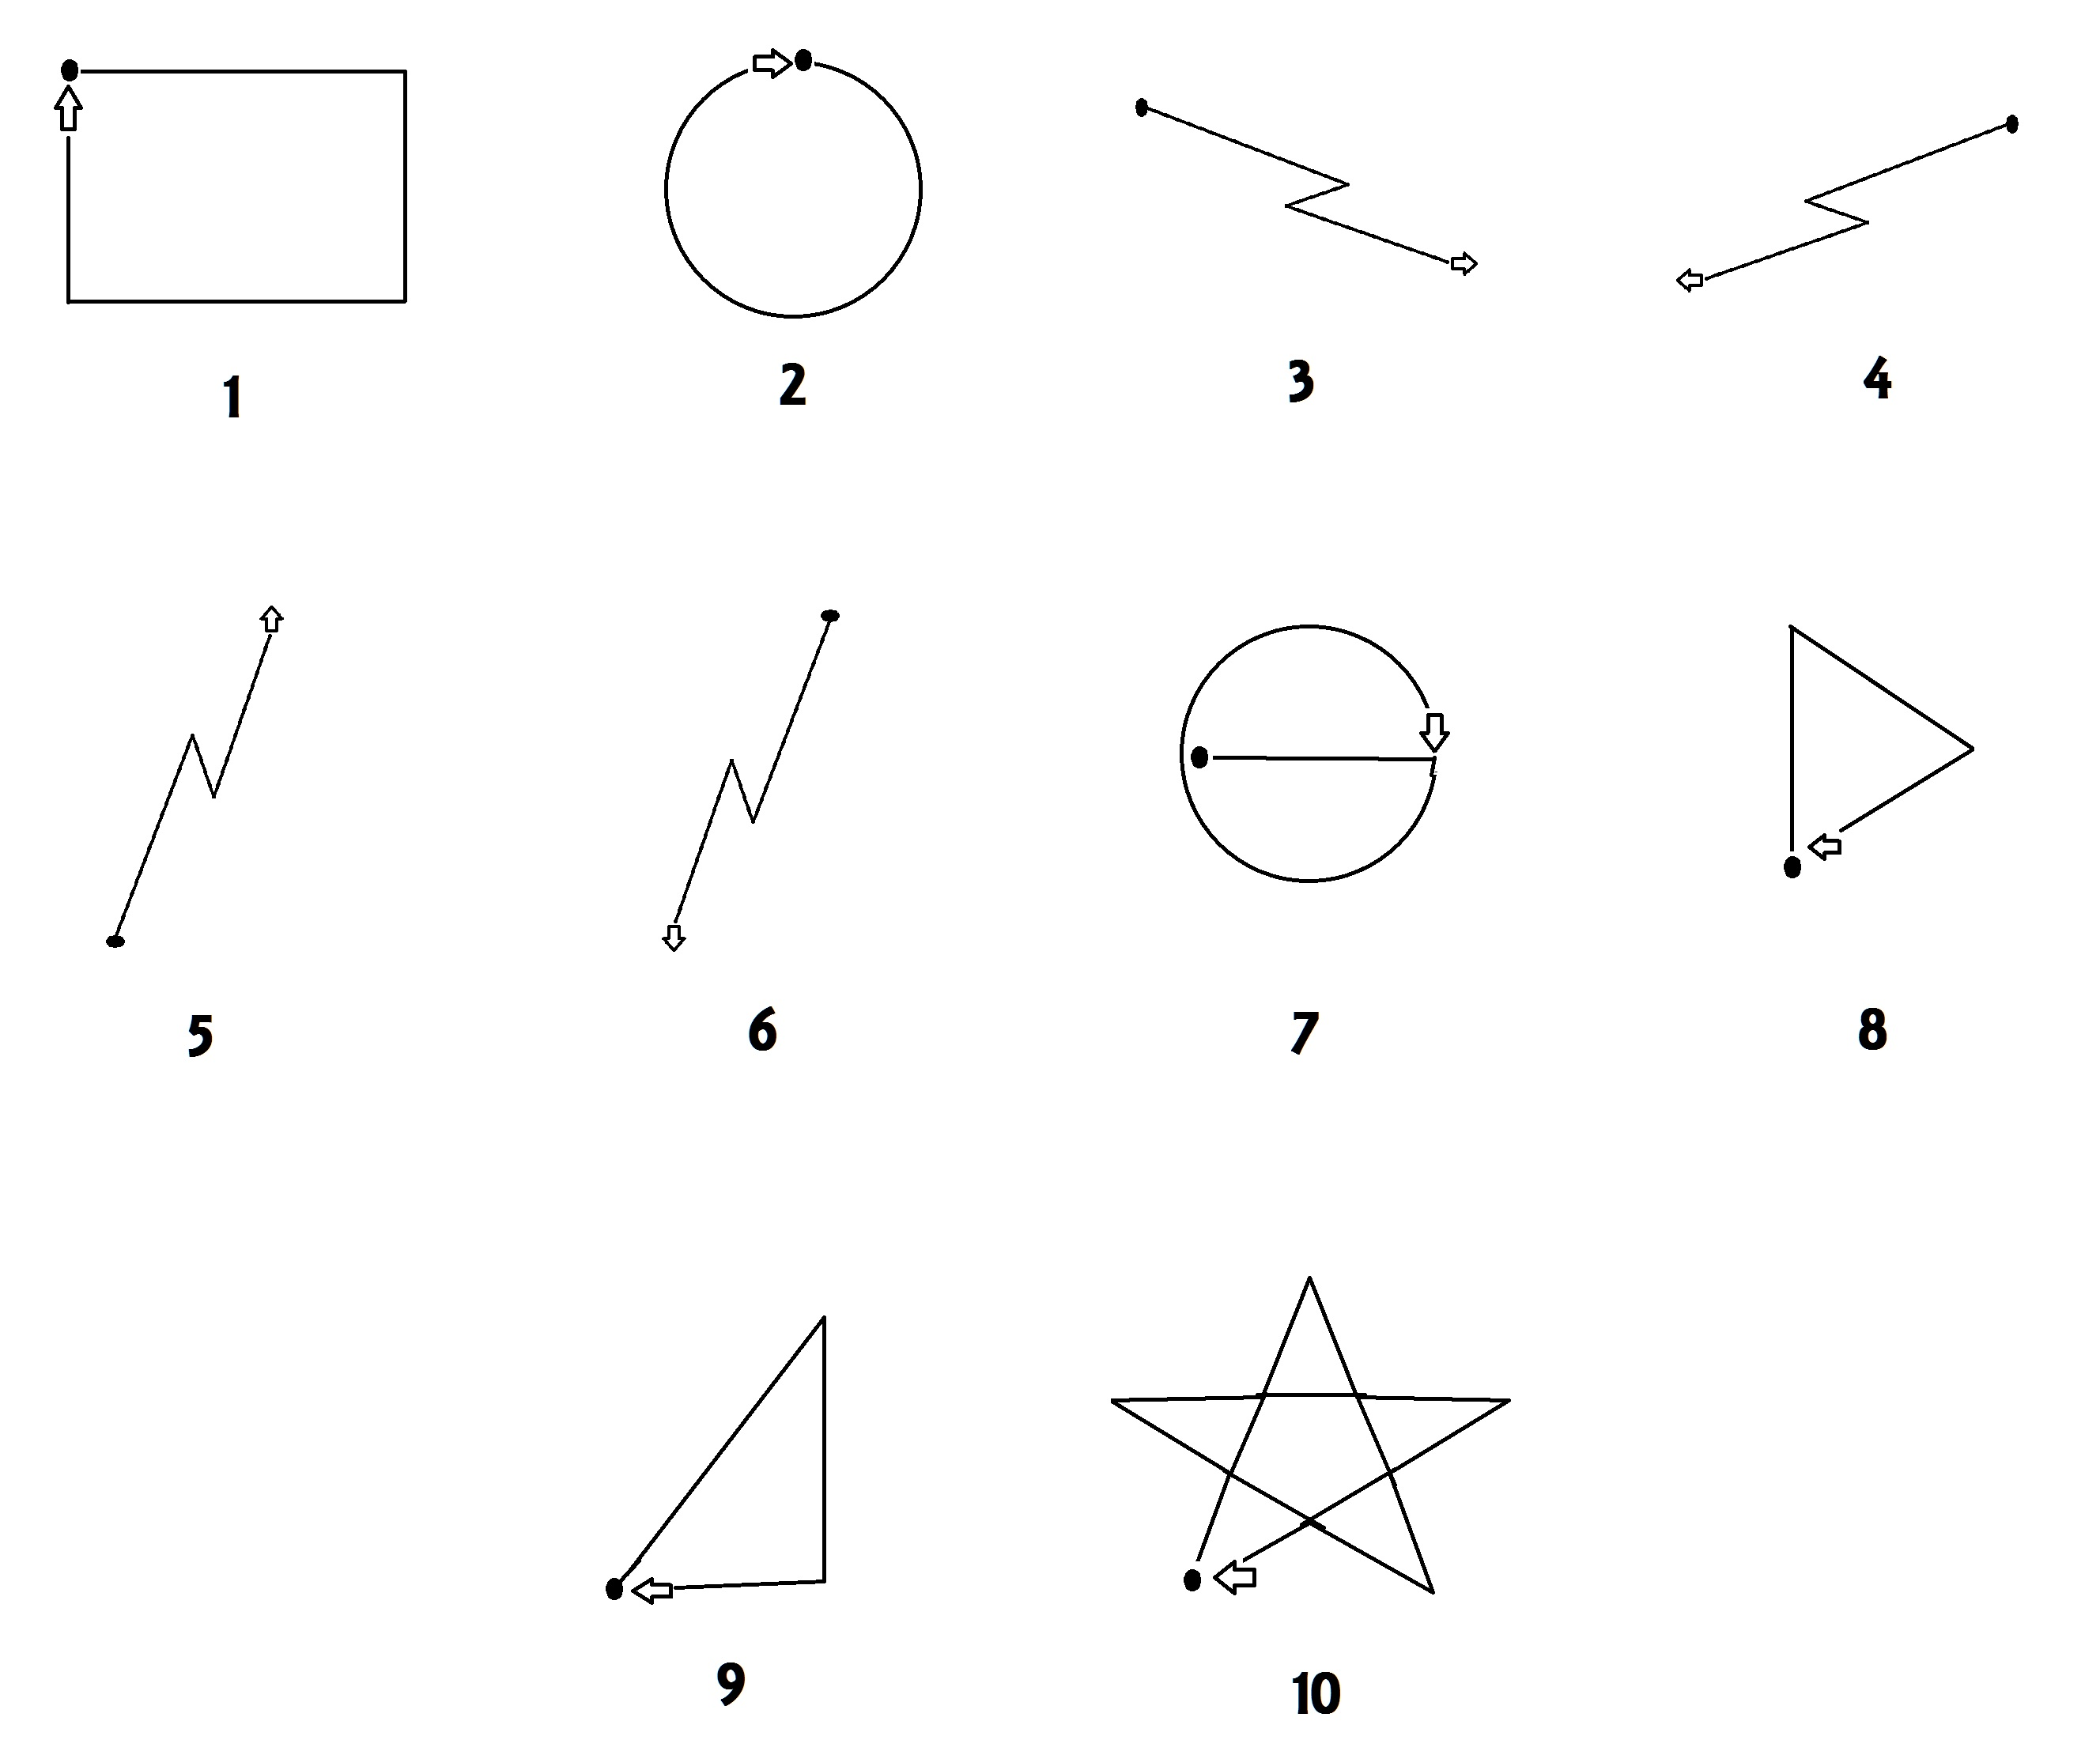
\includegraphics[width=\columnwidth]{Gestures}
  \caption{The gesture dictionary used for the HMM} \label{fig:Gestures}
\end{center}
\end{figure}

The acceleration and gyroscope data was obtained by means of an MPU6050 communicating with an Arduino Uno over an I2C communications protocol and MPU6050 library created by Jeff Rowberg \cite{Rowberg}. The Arduino was programmed to output the sensor data on the serial bus to a PC, which was parsed and dumped into user pre-defined files. The data files on the PC were then loaded into MATLAB where Kevin Murphy's HMM Toolbox for MATLAB \cite{Murphy} was utilized to train the HMM's for each gesture and to test the model with testing data. A parameter was used to vary the amount of training data and test data from the total data base of ten samples per gesture. 

Various experiments were performed to test the success of this algorithm for the task of gesture recognition of motion sensor data. Some of the tests that were performed included comparing how well gestures were recognized from a second user after training the model on only the first user, comparing the recognition rates of using only accelerometer data as opposed to using both accelerometer and gyroscope data, and the classification rate given different amounts of training data.




\section{Evaluation}
%	Evaluation - A section that quantitatively evaluates your ideas.
The sub sections below quantify and discuss the experiments utilizing the HMM for gesture recognition. These experiments offered supporting results for the analysis reviewed in Section III. For the purpose of representation of classifications of gestures, the concept of the Confusion matrix is shown in \TabRef{ConfMatrix}, with a single, correct classification for each gesture as an example. This matrix has a vertical axis correspondent to the true label of the gesture, while the horizontal axis represents the test case classification. The matrix can either represent the counts of classification or be normalized to represent probabilities of the classification. The off-diagonal entries of the Confusion matrix offer misclassification records. The matrix can be represented in either 2-D or 3-D format. Using this matrix, a classification error percentage can be calculated using the normalized difference in the sum of the total counts of the matrix and the off-diagonal entries.


	% Confusion Matrix
\begin{table}[h]
\renewcommand{\arraystretch}{1.2}
\caption{The Confusion Matrix for Testing Sets}
\label{tab:ConfMatrix}
\centering
\begin{tabular}{c||c|c|c|c|c|c|c|c|c|c|c}
\hline
    \hline
      & 1 & 2 & 3 & 4 & 5 & 6 & 7 & 8 & 9 & 10 & 11\\
    \hline    \hline
% Data goes here
    1 & 1 & 0 & 0 & 0 & 0 & 0 & 0 & 0 & 0 & 0 & 0\\
    \hline
    2 & 0 & 1 & 0 & 0 & 0 & 0 & 0 & 0 & 0 & 0 & 0\\
    \hline
    3 & 0 & 0 & 1 & 0 & 0 & 0 & 0 & 0 & 0 & 0 & 0\\
    \hline
    4 & 0 & 0 & 0 & 1 & 0 & 0 & 0 & 0 & 0 & 0 & 0\\
    \hline
    5 & 0 & 0 & 0 & 0 & 1 & 0 & 0 & 0 & 0 & 0 & 0\\
    \hline
    6 & 0 & 0 & 0 & 0 & 0 & 1 & 0 & 0 & 0 & 0 & 0\\
    \hline
    7 & 0 & 0 & 0 & 0 & 0 & 0 & 1 & 0 & 0 & 0 & 0\\
    \hline
    8 & 0 & 0 & 0 & 0 & 0 & 0 & 0 & 1 & 0 & 0 & 0\\
    \hline
    9 & 0 & 0 & 0 & 0 & 0 & 0 & 0 & 0 & 1 & 0 & 0\\
    \hline
    10 & 0 & 0 & 0 & 0 & 0 & 0 & 0 & 0 & 0 & 1 & 0\\
    \hline
    11 & 0 & 0 & 0 & 0 & 0 & 0 & 0 & 0 & 0 & 0 & 1\\
    \hline    \hline
\end{tabular}
\end{table}

\hfill



%%%%

\subsection{Multiple User Recognition}
Providing the HMM training sets from a single user, the test sets were almost entirely classified correctly as can be seen in \FigRef{User1}. This is the case when enough training data is supplied as compared to the amount of gestures.


\begin{figure}[h]
\begin{center}
\noindent
  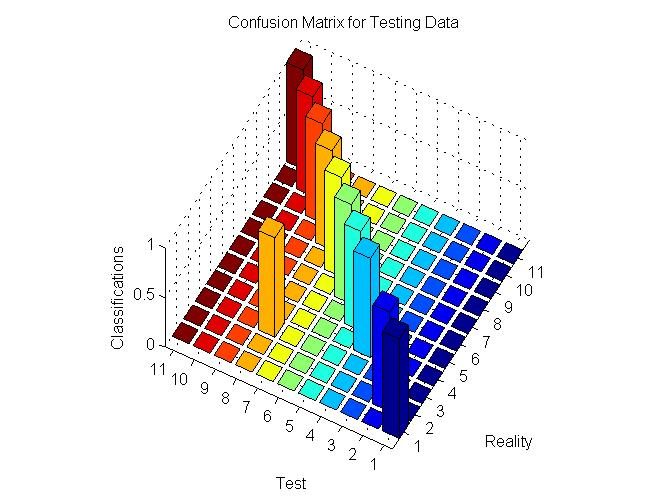
\includegraphics[width=\columnwidth]{User1}
  \caption{The Confusion Matrix for the Single User Training/Testing} \label{fig:User1}
\end{center}
\end{figure}

Contrary to the single user training and testing phase, training a HMM model with one user's gesture data, and subsequently testing the model with a different user's gestures causes what can be seen of in \FigRef{User2}. The misclassifications number significantly more than the single wrong test case in \FigRef{User1} as can be seen by the off diagonal entries. The reader should take note that the (1,1) entry is located in the bottom-right corner of the grid for viewing purposes. 


\begin{figure}[h]
\begin{center}
\noindent
  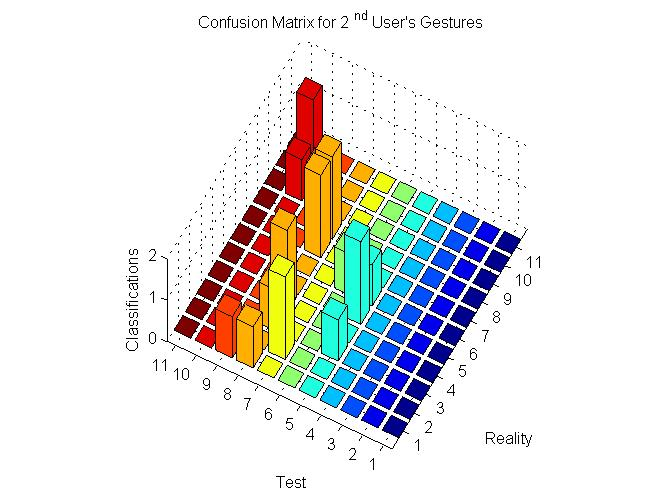
\includegraphics[width=\columnwidth]{User2}
  \caption{The Confusion Matrix for the $1^{st}$ User Training, $2^{nd}$ User Testing} \label{fig:User2}
\end{center}
\end{figure}

\hfill
%%%%


\subsection{Using Accel. vs. Accel. and Gyro. Data}
A comparison between the results of incorporating more sensor data, namely gyroscope data, in both the training and testing of the models showed that there was a significant decrease in the error rate of classification for the single user testing sets. The additional user, however, did not show considerable improvement across the range of training data percentage of the total data set supplied. Tabulated results are expressed in \TabRef{AvsAG}, where (only A) and (A \& G) signify the use of accelerometer data and both accelerometer and gyroscope data respectively.


\begin{table}[h]
\renewcommand{\arraystretch}{1.5}
\caption{The Accuracy Change with A vs. A/G over Training Data \%} \label{tab:AvsAG}
\centering
\resizebox{8cm}{!} {
\begin{tabular}{r l||c|c|c|c|c|c}
    \hline    \hline
    &  & 40\%  & 50\%  & 60\%  & 70\%  & 80\%  & 90\% \\
    \hline    \hline
% Data goes here
      (only A) & $ 1^{st}$ User & 45.46 & 27.28 & 13.64 & 15.15 & 13.64 & 0\\
     \hline
     (only A) & $2^{nd}$ User  & 80.00 & 70.00 & 65.00 & 60.00 & 55.00 & 70.00\\
     \hline     \hline
     (A \& G) & $1^{st}$ User & 62.12 & 30.91 & 13.64 & 3.03 & 4.55 & 9.10\\
     \hline
     (A \& G) & $2^{nd}$ User & 80.00 & 70.00 & 65.00 & 60.00 & 65.00 & 60.00\\
    \hline    \hline
\end{tabular}
}
\end{table}


%%%%

\subsection{Varying Amounts of Training Data}
For aiding in visualization, the data in \TabRef{VaryTrain} was taken from \TabRef{AvsAG} to show that the accuracy of classifications increases as the amount of training data increases. The optimal percentage of training data for this particular test run was around 70\%. The reason for this is most likely from the fact that the total sample set was limited to 10 samples per gesture and a training percentage of 70\% left 3 test cases per gesture, decreasing by 1 for every 10\% increase in the training percentage.


\begin{table}[h]
\renewcommand{\arraystretch}{1.5}
\caption{The Accuracy Change for Different Training Data \%} \label{tab:VaryTrain}
\centering
\resizebox{8cm}{!} {
\begin{tabular}{r l||c|c|c|c|c|c}
    \hline    \hline
    &  & 40\%  & 50\%  & 60\%  & 70\%  & 80\%  & 90\% \\
    \hline    \hline
% Data goes here
     (A \& G) & $1^{st}$ User & 62.12 & 30.91 & 13.64 & 3.03 & 4.55 & 9.10\\
    \hline    \hline
\end{tabular}
}
\end{table}
	
	
%%%%
	

\subsection{Run Time Variation}
The amount of time that the algorithm ran per the amount of training data percentage was compared over many iterations. The results in \TabRef{RunTimes} reveal that the relationship for these test cases was linear. Since the data sets only incorporated a total of 10 samples per gesture, the training percentage corresponds to providing 1 additional training set per 10 percentage points. For a more thorough investigation of the runtime, training data amounts spanning many orders of magnitude would be necessary.

\begin{table}[h]
\renewcommand{\arraystretch}{1.5}
\caption{The Run Times for Different Training Data \%} \label{tab:RunTimes}
\centering
\begin{tabular}{c||c|c|c|c|c|c}
    \hline    \hline
                             & 40\%  & 50\% & 60\% & 70\% & 80\% & 90\%\\
    \hline
% Data goes here
     Time (s): Run 1 & 57.9 & 68.4 & 87.8 & 97.3 & 128.3 & 129.0\\
     \hline
     Time (s): Run 2 & 58.7 &  70.9  & 88.7  &100.3 & 115.2 & 140.6\\
    \hline    \hline
\end{tabular}
\end{table}
\hfill

% Training data ranging from 40% to 90%
%missclass =
%
%   31.8182         70.0000      26.9231
%   25.4545         70.0000     21.5385
%   13.6364         55.0000      13.0769
%   12.1212         55.0000     11.5385
%         0             70.0000      10.7692
%    9.0909          50.0000        8.4615
%    
%    missclass =
%
%   45.4545   80.0000   53.4884
%   27.2727   70.0000   38.6667
%   13.6364   65.0000   29.6875
%   15.1515   60.0000   32.0755
%   13.6364   55.0000   33.3333
%         0   70.0000   45.1613
%
%
%Adding the Gyro data and sweeping from 40-90% training data
%missclass =
%
%   39.3939   60.0000   44.1860
%   16.3636   65.0000   29.3333
%   11.3636   55.0000   25.0000
%    6.0606   50.0000   22.6415
%    9.0909   75.0000   40.4762
%    9.0909   60.0000   41.9355
%    
%    missclass =
%
%   62.1212   80.0000   66.2791
%   30.9091   70.0000   41.3333
%   13.6364   65.0000   29.6875
%    3.0303   60.0000   24.5283
%    4.5455   65.0000   33.3333
%    9.0909   60.0000   41.9355




\section{Conclusion}
%	Summary and Conclusions - Summarize what you did and what interesting things you learned from the project.

The area of gesture recognition is large in application bases. This study both reviewed some of the previous and current means of performing this task, as well as presented the HMM algorithm approach towards solving the gesture recognition problem. Many different experiments were performed to include comparing classification rates by processing another user's gestures through a model trained by a different user's gesture data. It was seen that the HMM is sensitive to specific user training. Adding additional data per training set from the gyroscope measurements provides lowered classification error, and varying the amount of training data supplied to the models directly lowered the error rates for both the single user and double user tests. Additionally, some quick run time analysis was performed to see that the HMM runs in approximately linear time over the percentage of the training data from the entire data set. It should be noted that to perform a true run time analysis, many separate orders of magnitude of data sets should be used in stead of the 10 used for this study.

For future work, a comparative analysis of each algorithm reviewed in this paper could be done. While the different strengths and weaknesses of each algorithm have already been discussed here and in other papers, a concise representation of all algorithm performances could provide a means to chose which algorithm best fits an application area. Additional focus could be implemented within the data pre-processing phase to help eliminate measurement noise to aid in better model formulation. Since adding the gyroscope data provided lower classification error for a single user's test sets without addition of significant computation time, experimenting with other types of additional data for the training sets would be a future focus as well.  


% references section

% can use a bibliography generated by BibTeX as a .bbl file
% BibTeX documentation can be easily obtained at:
% http://www.ctan.org/tex-archive/biblio/bibtex/contrib/doc/
% The IEEEtran BibTeX style support page is at:
% http://www.michaelshell.org/tex/ieeetran/bibtex/
%\bibliographystyle{IEEEtran}
% argument is your BibTeX string definitions and bibliography database(s)
%\bibliography{IEEEabrv,../bib/paper}
%
% <OR> manually copy in the resultant .bbl file
% set second argument of \begin to the number of references
% (used to reserve space for the reference number labels box)
\begin{thebibliography}{7}

\bibitem{DTW}
Akl, A.; Valaee, S., "Accelerometer-based gesture recognition via dynamic-time warping, affinity propagation, \& compressive sensing," \emph{Acoustics Speech and Signal Processing (ICASSP), 2010 IEEE International Conference on}, vol., no., pp.2270,2273, 14-19 March 2010,doi: 10.1109/ICASSP.2010.5495895
%keywords: {accelerometers;gesture recognition;statistical analysis;accelerometer-based gesture recognition;affinity propagation;compressive sensing;dynamic-time warping;single 3-axis accelerometer;statistical methods;user-dependent recognition;Acceleration;Accelerometers;Computer interfaces;Databases;Dictionaries;Hidden Markov models;Humans;Pattern recognition;Statistical analysis;Testing;affinity propagation;compressive sensing;dynamic time warping;gesture recognition},
%URL: http://ieeexplore.ieee.org/stamp/stamp.jsp?tp=&arnumber=5495895&isnumber=5494886

\bibitem{Kling}
Klingmann, Marco. "Accelerometer-based gesture recognition with the iphone." Master's thesis, Goldsmiths University of London (2009).


\bibitem{SFA}
Koch, P.; Konen, W.; Hein, K., "Gesture recognition on few training data using Slow Feature Analysis and parametric bootstrap," \emph{Neural Networks (IJCNN), The 2010 International Joint Conference on}, vol., no., pp.1,8, 18-23 July 2010,doi: 10.1109/IJCNN.2010.5596842
%keywords: {feature extraction;gesture recognition;image classification;unsupervised learning;Bluetooth Wiimote controller;Nintendo;gesture recognition;nonlinear function space;parametric bootstrap;random forest predictor;slow feature analysis;time series classification;training data;Accelerometers;Error analysis;Gesture recognition;Radio frequency;Sensors;Training;Training data},
%URL: http://ieeexplore.ieee.org/stamp/stamp.jsp?tp=&arnumber=5596842&isnumber=5595732



\bibitem{FSM}
Mitra S.; Acharya T., "Gesture Recognition: A Survey," \emph{Systems, Man, and Cybernetics, Part C: Applications and Reviews, IEEE Transactions on}, vol.37, no.3, pp.311,324, May 2007,doi: 10.1109/TSMCC.2007.893280
%keywords: {face recognition;finite state machines;gesture recognition;hidden Markov models;human computer interaction;image colour analysis;image sequences;condensation;connectionist models;facial expressions;finite-state machines;gesture recognition;hand gestures;hidden Markov models;intelligent human-computer interface;optical flow;particle filtering;skin color;Arm;Face recognition;Filtering;Handicapped aids;Hidden Markov models;Humans;Magnetic heads;Manifolds;Optical filters;Virtual reality;Face recognition;facial expressions;hand gestures;hidden Markov models (HMMs);optical flow;soft computing},
%URL: http://ieeexplore.ieee.org/stamp/stamp.jsp?tp=&arnumber=4154947&isnumber=4154935



\bibitem{Rowberg}
Rowberg J. (2014, April 10). \emph{MPU-6050 6-axis accelerometer/gyroscope} [Online]. Available: http://www.i2cdevlib.com/devices/mpu6050



\bibitem{Murphy}
Murphy K. (2005, June 5). \emph{Hidden Markov Models (HMM) Toolbox for MATLAB} [Online]. Available: http://www.cs.ubc.ca/\~{}murphyk/Software/HMM/hmm.html

\bibitem{Many}
Wood D. (2014, April 15). \emph{Multi-touch Gesture Recognition for Games} [Online]. Available: http://people.cs.uct.ac.za/~nschiff/ipadGame/pdfs/danielReport.pdf


\end{thebibliography}




\end{document}



%Instructions for Preparing Your Project Reports
%•	The length of a report must be no more than 10 pages.

%•	Reports must include the following parts:
%o	Project title and your name
%o	Abstract - A paragraph that summarizes the problem and the results.
%o	Introduction - Sets the context, describes the problem, and describes your solution.
%o	Description - One or more sections that describes the problem and your approach to the solution in detail.
%o	Evaluation - A section that quantitatively evaluates your ideas.
%o	Related work - Describes representative works related to your work, and summarizes the pros and cons of each work.
%o	Summary and Conclusions - Summarize what you did and what interesting things you learned from the project.
%o	Reference list
%
%•	You also need to submit your computer programs that you develop for your project.
%•	In addition, you need to prepare a Powerpoint file, which must include the following parts (there is no page limit for the Powerpoint file):
%o	The problem under study
%o	Existing approaches
%o	(Optional) Proposed new approach if there is any
%o	Performance evaluation of existing approaches and (if any) the proposed new approach
%o	Conclusion





%Criteria Used for Grading Your Project Report
%1.	Quality. The value of a paper is a function of the innate character or degree of excellence of the work described. Was the work performed, or the study made with a high degree of thoroughness? Was high engineering skill demonstrated? Is an experiment described which has a high degree of elegance? Or, on the other hand, is the work described pretty much of a run-of-the-mill nature? 
%2.	Presentation. The value of the paper is a function of the ease with which the reader can determine what the author is trying to present. Regardless of the other criteria, a paper is not good unless the material is presented clearly and effectively. Is the paper well written? Is the meaning of the author clear? Are the tables, charts and figures clear? Is their meaning readily apparent? Is the information presented in the paper complete? At the same time, is the paper concise?
%3.	(Bonus) Originality. The value of a paper is a function of the degree to which it presents new or novel technical material. Does the paper present results previously unknown? Does it push forward the frontiers of knowledge? Does it present new methods for solving old problems or new viewpoints on old problems? Or, on the other hand, is it a re-hash of information already known?
%4.	(Bonus) Contribution. The value of a paper is a function of the degree to which it represents an overall contribution to the advancement of the art. This is different from originality. A paper may be highly original, but may be concerned with a very minor, or even insignificant, matter or problem. On the other hand, a paper may make a great contribution by collecting and analyzing known data and facts and pointing out their significance. Or, a fine exposition of a known, but obscure or complex, phenomenon or theory or system or operating technique may be a very real contribution to the art. Obviously, a paper may well score highly on both originality and contribution. Perhaps a significant question is, will the engineer who reads the paper be able to practice his profession more effectively because of having read it?

